\documentclass[10pt,a4paper,spanish]{article}

\usepackage[spanish]{babel}
\usepackage[utf8]{inputenc}
\usepackage{amsmath, amsthm}
\usepackage{amsfonts, amssymb, latexsym}
\usepackage{enumerate}
\usepackage[official]{eurosym}
\usepackage{graphicx}
\usepackage[usenames, dvipsnames]{color}
\usepackage{colortbl}
\usepackage{multirow}
\usepackage{fancyhdr}
\usepackage{fancybox}
\usepackage{pseudocode}
\usepackage[all]{xy}
\usepackage{minted}
\usepackage{tikz}
\usepackage{pgfplots}

\pgfplotsset{compat=1.5}

% a4large.sty -- fill an A4 (210mm x 297mm) page
% Note: 1 inch = 25.4 mm = 72.27 pt
%       1 pt = 3.5 mm (approx)

% vertical page layout -- one inch margin top and bottom
\topmargin      0 mm    % top margin less 1 inch
\headheight     0 mm    % height of box containing the head
\headsep       10 mm    % space between the head and the body of the page
\textheight   250 mm
\footskip      14 mm    % distance from bottom of body to bottom of foot

% horizontal page layout -- one inch margin each side
%\oddsidemargin    0   mm    % inner margin less one inch on odd pages
%\evensidemargin   0   mm    % inner margin less one inch on even pages
%\textwidth      159.2 mm    % normal width of text on page

\usepackage[math]{iwona}
\usepackage[T1]{fontenc}
\usepackage{inconsolata}

\usepackage[pdftex, bookmarks=true,
bookmarksnumbered=false, % true means bookmarks in
% left window are numbered
bookmarksopen=false,     % true means only level 1
% are displayed.
colorlinks=true,
linkcolor=webblue]{hyperref}

\definecolor{webgreen}{rgb}{0, 0.5, 0} % less intense green
\definecolor{webblue}{rgb}{0, 0, 0.5}  % less intense blue
\definecolor{webred}{rgb}{0.5, 0, 0}   % less intense red
\definecolor{dblackcolor}{rgb}{0.0,0.0,0.0}
\definecolor{dbluecolor}{rgb}{.01,.02,0.7}
\definecolor{dredcolor}{rgb}{0.8,0,0}
\definecolor{dgraycolor}{rgb}{0.30,0.3,0.30}

\newcommand{\HRule}{\rule{\linewidth}{0.5mm}} % regla horizontal para  el titulo

\pagestyle{fancy}
%con esto nos aseguramos de que las cabeceras de capítulo y de sección vayan en minúsculas

\renewcommand{\chaptermark}[1]{%
\markboth{#1}{}}
\renewcommand{\sectionmark}[1]{%
\markright{\thesection\ #1}}
\fancyhf{} %borra cabecera y pie actuales
\fancyhead[LE,RO]{\bfseries\thepage}
\fancyhead[LO]{\bfseries\leftmark}
\renewcommand{\headrulewidth}{0.5pt}
\renewcommand{\footrulewidth}{0pt}
\addtolength{\headheight}{0.5pt} %espacio para la raya
\fancypagestyle{plain}{%
\fancyhead{} %elimina cabeceras en páginas "plain"
\renewcommand{\headrulewidth}{0pt} %así como la raya
}

%%%%% Para cambiar el tipo de letra en el título de la sección %%%%%%%%%%%
\usepackage{sectsty}
\chapterfont{\fontfamily{pag}\selectfont} %% for chapter if you want
\sectionfont{\fontfamily{pag}\selectfont}
\subsectionfont{\fontfamily{pag}\selectfont}
\subsubsectionfont{\fontfamily{pag}\selectfont}

\renewcommand{\labelenumi}{\arabic{enumi}. }
\renewcommand{\labelenumii}{\alph{enumii}) }
\renewcommand{\labelenumiii}{\labelenumii\roman{enumiii}: }

\begin{document}
  \setcounter{section}{0}
  \title{\huge\bf Informática Industrial \\ Relación de Ejercicios Nº 3}
  \author{\large David Sánchez Jiménez}
  \maketitle
  \vspace{3cm}

  \begin{enumerate}
    \item ¿Qué es una RTU? Principales características y ejemplos.

    \noindent
    Un RTU (Remote Terminal Unit) es un dispositivo basado en microprocesadores, el cual permite obtener señales independientes de los procesos y enviar la información a una estación maestra donde se procese. Tambien puede usar información de la estación maestra para aplicarlo en algun proceso que realice. Puede tener canales de control o sensores de entrada, dispositivos de información en el mismo RTU, alarmas o puertos de comunicación. \\

    \noindent
    Algunos ejemplos de RTU son los siguientes:
    \begin{itemize}
      \item ROC800-Series Remote Operations Controller
      \item FloBoss 107 Distributed RTU
      \item A6328 Distributed RTU Network


    \end{itemize}

    \item ¿En qué consiste el control basado en PC (Slot-PLC y Soft-PLC)?

    \noindent
    El control basado en PC consiste en usar sistemas basados en PC sustituyendo a los PLC.

    \begin{itemize}
      \item Slot-PLC: Consiste en realizar un PLC en una placa de circuito impreso la cual se coloca en un slot del bus principal del PC. Sus características principales son la alimentación independiente del computador para mayor robustez ante cualquier fallo del PC, una arquitectura más económica que utilizar un PLC independiente, conexión a los dispositivos de campo, mayor velocidad y fiabilidad en el intercambio de información PC-PLC.

      \item Soft-PLC: Son aplicaciones informáticas que, en combinación con algu RTOS emulan mediante Software el funcionamiento de un PLC. Este sistema se programa y se comporta igual que un PLC.
    \end{itemize}

    \newpage
    \item Indicar los principales elementos hardware de un PLC.

    \noindent
    Los principales elementos hardware de un PLC son:

    \begin{itemize}
      \item CPU
      \item Fuente de Alimentación
      \item Memoria RAM, EPROM, EEPROM (Flash)
      \item Entradas/Salidas analógicas, digitales y contadores rápidos.
      \item Comunicación RS-232, RS-485, buses de campo, Ethernet, fibra óptica.
      \item Módulos de control de motores, lógica fuzzy, visión artificial...
    \end{itemize}

    \item Dibuje y describa el diagrama del ciclo de funcionamiento de un PLC.

    \noindent
    \begin{figure}[!hbp]
      \centering  \includegraphics[width=1\textwidth]{./Imagenes/1.png}
    \end{figure}


    \item Indicar los principales lenguajes de programación de un PLC.

    \noindent
    Los principales lenguajes de programación de un PLC son:

    \begin{itemize}
      \item Diagrama de Bloques de Funciones (FBD)
      \item Sequential Flow Chart (SFC)
      \item Diagrama Ladder (LD)
      \item Lista de instrucciones (IL)
      \item Texto estructurado (ST)
      \item GRAFCET
    \end{itemize}

    \newpage
    \item Se dispone de un tanque de agua con una válvula de entrada y otra de salida (ambas de tipo todo-nada), detector de temperatura baja, un detector de nivel máximo, y una resistencia calefactora de tipo todo-nada. Se desea diseñar un sistema de control con PLC de forma que:
    \begin{itemize}
      \item La válvula de entrada se deberá abrir cuando el nivel es bajo.
      \item La válvula de entrada se deberá cerrar cuando el nivel es alto.
      \item El calefactor se deberá conectar cuando la temperatura es baja y desconectar cuando no lo es.
      \item La válvula de salida se abrirá cuando el tanque esté lleno y la temperatura sea alta. En caso de que fallen los detectores de nivel, y ambos estén activos a la vez, se cerrará la válvula de entrada, se abrirá la de salida y se encenderá una luz roja de alarma.
    \end{itemize}

    \begin{enumerate}
      \item Dibujar un esquema sinóptico del sistema, que incluya el proceso, los detectores, actuadores, y las entradas y salidas del PLC.

      \begin{figure}[!hbp]
        \centering  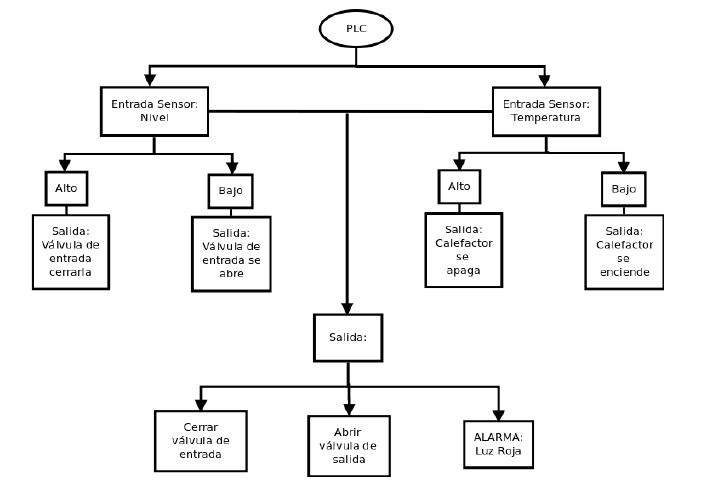
\includegraphics[width=1\textwidth]{./Imagenes/2.png}
      \end{figure}

      \newpage
      \item Realizar un diagrama de GRAFCET del mismo.

      \begin{figure}[!hbp]
        \centering  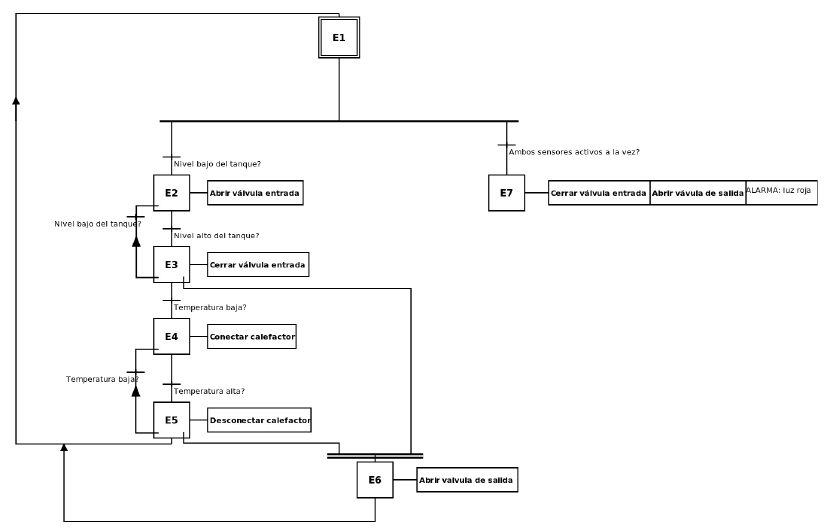
\includegraphics[width=1\textwidth]{./Imagenes/3.png}
      \end{figure}


    \end{enumerate}

    \item Describe los principales tipos de sistemas de visualización que se usan en centros de control.

    \noindent
    Los principales tipos de sistemas de visualización que se usan en centros de control son:

    \begin{itemize}
      \item Video Wall: Ya sea mediante la retroproyección sobre una pantalla en un cubo, con una matriz de pantallas planas o con una composición de pantallas en forma de mosaico.
      \item Pantallas UltraRes con pantalla tactil y una resolución 4K.
      \item Pantallas LED de gran dimensión pero con baja resolución.
    \end{itemize}

    \item Indique qué es un sistema SCADA y cuáles son sus funciones básicas.

    \noindent
    Un sistema SCADA es un software que permite controlar y supervisar procesos industriales a distancia facilitando la retro-alimentación en tiempo real con los dispositivos de campo y controlando los procesos automáticamente. El sistema SCADA nos provee de toda la información que se genera en el proceso productivo y permite su gestión e intervención.

    \item Describa los tipos de alarmas de un software SCADA.

    \noindent
    Las alarmas pueden ser de varios tipos segun sus características:
    \begin{itemize}
      \item Discretas: Cambian un tag de 0 a 1 o a la inversa.
      \item Desviación: Se activan cuando el tag se desvia por encima o debajo del valor específicado.
      \item Valor: alto, bajo, muy alto, muy bajo.
      \item Frecuencia de Cambio: Cuando el tag cambia de valor un numero excesivo de veces en un tiempo prefijado.
    \end{itemize}

    \item ¿Qué es un OPC?

    \noindent
    El OPC(OLE for Process Control) es un estándar de comunicación en el campo del control y supervisión de procesos industriales, basado en una tecnología Microsoft, que ofrece una interfaz común para comunicación que permite que componentes software individuales interactúen y compartan datos. El servidor OPC es la fuente de datos (como un dispositivo hardware a nivel de planta) y cualquier aplicación basada en OPC puede acceder a dicho servidor para leer/escribir cualquier variable que ofrezca el servidor.
  \end{enumerate}


\end{document}
